\chapter{有限元法}

\section{有限元法概述}

\par 首先简单地介绍加权残差法,然后求解一个简单的一维 Helmholtz 方程,以此来阐明
有限元法的基本原理。

\subsection{一般原理}

\par 使用加权残差法或变分法均可以建立有限元法的公式。在本章中,我们使用加权残
差法。

\par 考虑如下的偏微分方程:
\begin{equation}
    \mathcal{L}\varphi = f
    \label{偏微分方程}
\end{equation}
\par 式中,$\mathcal{L}$ 为微分算子,
$\varphi$ 为待求未知解,$f$ 为源函数。为了求得 $\varphi$ 的解,用一组基函
数将其展开:
\begin{equation}
    \varphi = \sum_{j=1}^{N} c_j v_j
    \label{基函数展开}
\end{equation}
\par 其中 $c_j$ 为待求系数,$v_j$ 为基函数。
将式 (\ref{基函数展开}) 代入式 (\ref{偏微分方程}) 中,
然后将得到的等式乘以加权
函数 $w_i$,并在整个求解区域 $\Omega$ 中积分得到:
\begin{equation}
    \int_{\Omega} w_i \mathcal{L}\left(\sum_{j=1}^{N} c_j v_j\right)
     \text{d}\Omega = \int_{\Omega} w_i f \text{d}\Omega
    \label{加权残差法}
\end{equation}
\par 当给定一组加权函数,上式就定义了一个代数方程组,
在满足边界条件的要求下求解此方程
组即可得到 $c_j$。

\begin{theorem}{Galerkin 法}
    当加权函数与基函数相等时,即 $w_i = v_i$,
    式 (\ref{加权残差法}) 变成
    \begin{equation}
        \int_{\Omega} v_i \mathcal{L}\left(\sum_{j=1}^{N} c_j v_j\right)
        \text{d}\Omega = \int_{\Omega} v_i f \text{d}\Omega
        \qquad i = 1, 2, \cdots, N
    \end{equation}
    将其写为矩阵形式
    \begin{equation}
        \sum_{j=1}^{N} S_{ij} c_j = b_i \qquad i = 1, 2, \cdots, N
    \end{equation}
    其中
    \begin{align}
        S_{ij} &= \int_{\Omega} v_i \mathcal{L} v_j \text{d}\Omega \\
        b_i &= \int_{\Omega} v_i f \text{d}\Omega
    \end{align}
\end{theorem}

\par 在构建公式的过程中,最关键的一步是找到一组可以用来展开未知解的基函数。对于复杂
的具有不规则形状的二维和三维问题,这是极其困难甚至不可能的。
有限元法的基本思想是将
求解区域划分为小的子域,称为有限单元,然后使用简单的函数,如线性函数或二次
函数来近似每个单元内的未知解。

\subsection{一维算例}

\par 考虑一个 Helmholtz 方程的一维边值问题:
\begin{equation}
    \frac{\text{d}^2\varphi}{\text{d}x^2} + k^2\varphi = f
    \qquad 0<x<L
    \label{一维Helmholtz}
\end{equation}
\par 其边界条件为
\begin{align}
    \label{一维边界条件-1}
    \left.\varphi\right|_{x=0} &= p \\
    \label{一维边界条件-2}
    \left.\left(
        \frac{\text{d}\varphi}{\text{d}x} + \gamma\varphi
    \right)\right|_{x=L} &= q
\end{align}

\begin{figure}[!htbp]
    \centering
    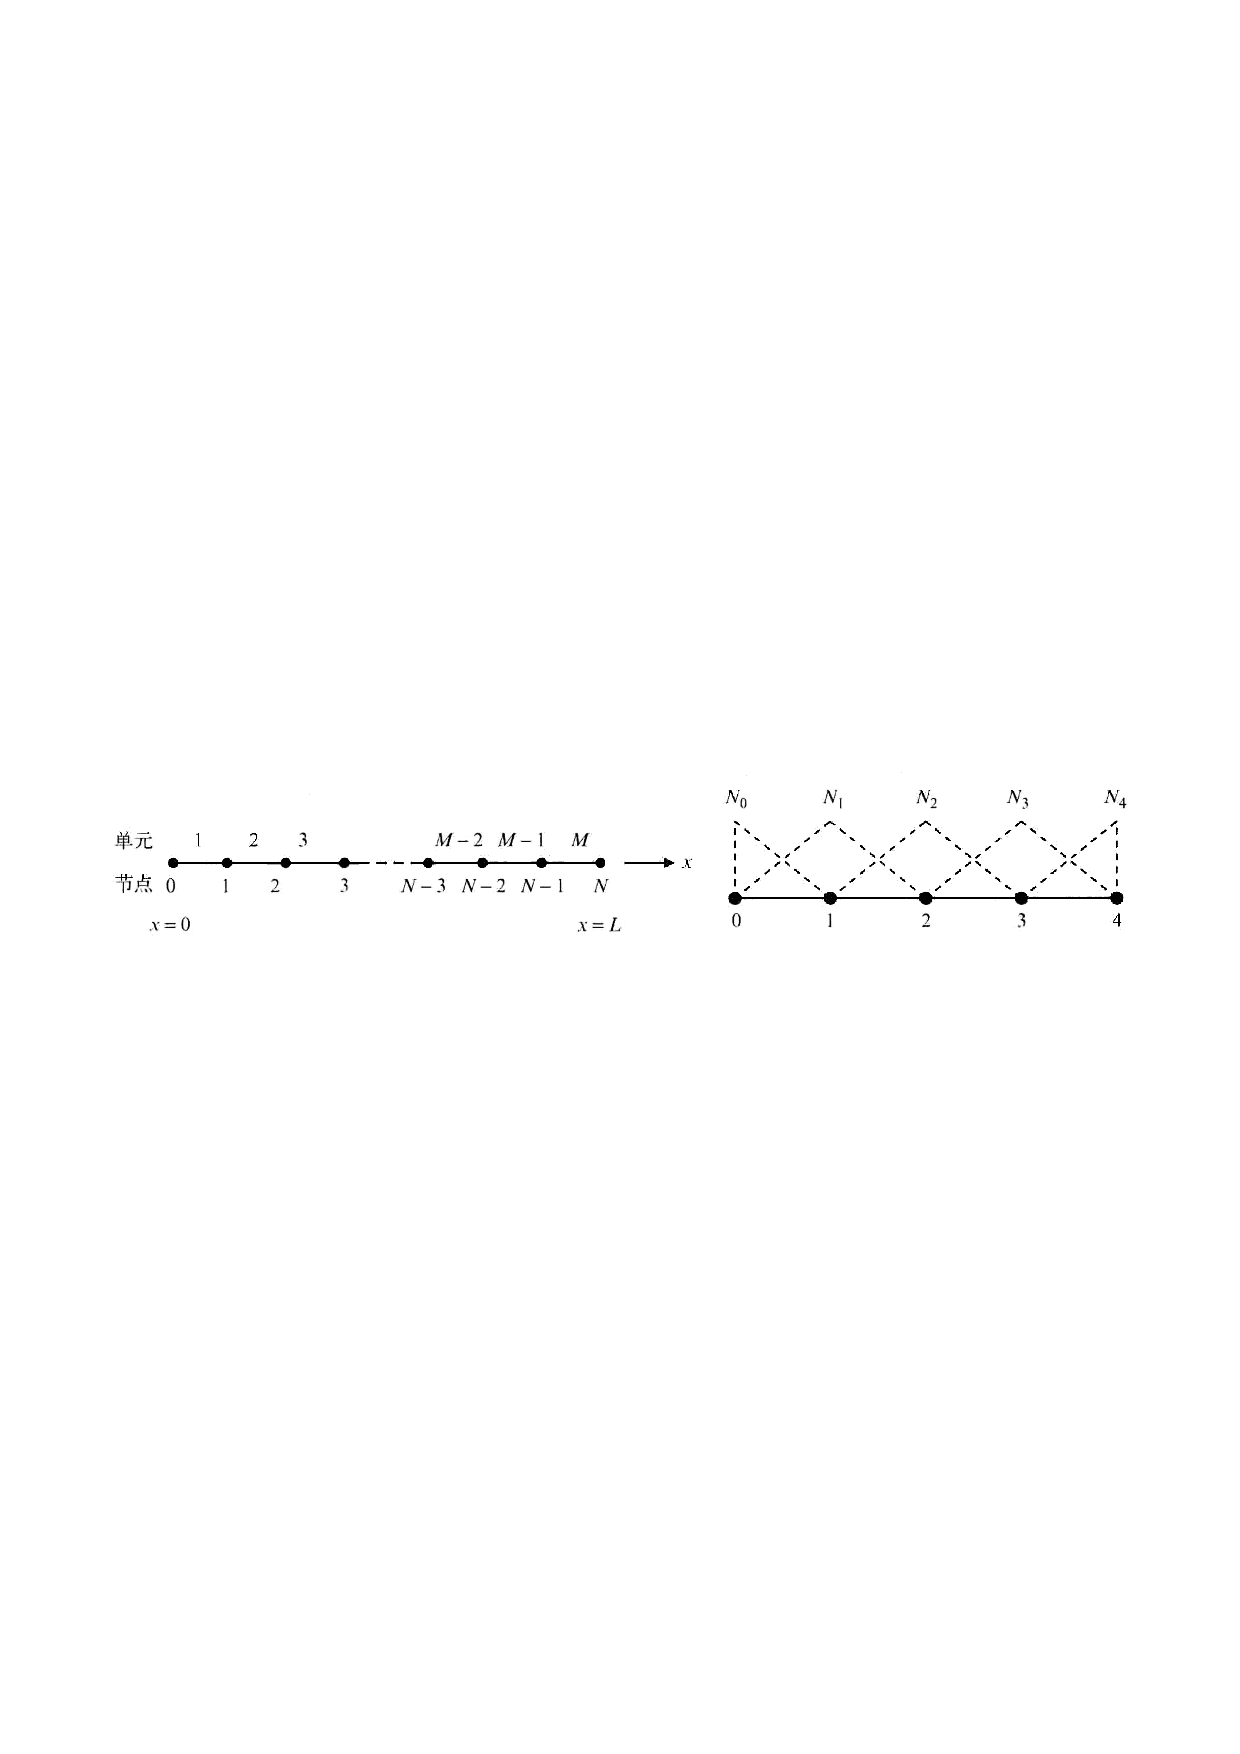
\includegraphics[scale=0.95]{3.1.2-1.pdf}
    \caption{一维网格和一维线性基函数}
    \label{一维网格和一维线性基函数}
\end{figure}

\par 有限元法的第一步是将求解区域 $(0,L)$ 划分成多个单元。
我们让单元
足够小,使得每个单元上的未知解可以通过对此单元两端节点上的值进行线性插值得到。
于是,未知解可表示为
\begin{equation}
    \varphi(x) = \sum_{j=0}^{N} \varphi_j N_j(x)
    =\sum_{j=1}^{N} \varphi_j N_j(x)
    +\varphi_0 N_0(x)
    =\sum_{j=1}^{N} \varphi_j N_j(x)
    +p N_0(x)
    \label{一维基函数展开}
\end{equation}
\par 其中 $\varphi_j$ 为未知量在第 $j$ 个节点处的值,
$N_j(x)$ 为相应的基函数。
$N_j(x)$ 是一个三角形函数,仅在第 $j$ 个单元与第 $j+1$ 个单
元上具有非零值。

\begin{theorem}{Galerkin 法}{一维算例 Galerkin 法}
    对于该一维 Helmholtz 方程,我们可以得到如下方程组
    \begin{equation}
        \sum_{j=1}^{N} K_{ij} \varphi_j = b_i \qquad i = 1, 2, \cdots, N
    \end{equation}
    其中
    \begin{align}
        K_{ij} &= 
        \int_{0}^{L}\left[
            \frac{\text{d}N_i(x)}{\text{d}x}\frac{\text{d}N_j(x)}{\text{d}x}
            - k^2N_i(x)N_j(x)
        \right]\text{d}x+\gamma\delta_{iN}\delta_{jN}\\
        b_i &= 
        -\int_{0}^{L}N_i(x)f(x)\text{d}x
        -p\int_{0}^{L}\left[
            \frac{\text{d}N_i(x)}{\text{d}x}\frac{\text{d}N_0(x)}{\text{d}x}
            - k^2N_i(x)N_0(x)
        \right]\text{d}x+q\delta_{iN}
    \end{align}
\end{theorem}

\begin{exercise}
    推导上述方程组。
\end{exercise}

\begin{solution}
    由 Galerkin 法,我们有
    \begin{equation*}
        \int_{0}^{L}N_i(x)\left[
            \frac{\text{d}^2\varphi(x)}{\text{d}x^2}+k^2\varphi(x)
        \right]\text{d}x = 
        \int_{0}^{L}N_i(x)f(x)\text{d}x
    \end{equation*}
    使用分部积分,得到
    \begin{gather*}
        \int_{0}^{L}N_i(x)
        \text{d}\left(\frac{\text{d}\varphi(x)}{\text{d}x}\right) 
        +\int_{0}^{L}
            k^2N_i(x)\varphi(x)
        \text{d}x = 
        \int_{0}^{L}N_i(x)f(x)\text{d}x\\
        \left.\left(
            N_i(x)\frac{\text{d}\varphi(x)}{\text{d}x}
        \right)\right|_0^L
        -\int_{0}^{L}
        \frac{\text{d}N_i(x)}{\text{d}x}
        \frac{\text{d}\varphi(x)}{\text{d}x}
        \text{d}x
        +\int_{0}^{L}
            k^2N_i(x)\varphi(x)
        \text{d}x = 
        \int_{0}^{L}N_i(x)f(x)\text{d}x\\
        \int_{0}^{L}\left[
            \frac{\text{d}N_i(x)}{\text{d}x}\frac{\text{d}\varphi(x)}{\text{d}x}
            - k^2N_i(x)\varphi(x)
        \right]\text{d}x
        -\left[N_i(x)\frac{\text{d}\varphi(x)}{\text{d}x}\right]_{x=L} = 
        -\int_{0}^{L}N_i(x)f(x)\text{d}x
    \end{gather*}
    将式 (\ref{一维边界条件-2}) 代入上式,得到
    \begin{equation*}
        \int_{0}^{L}\left[
            \frac{\text{d}N_i(x)}{\text{d}x}\frac{\text{d}\varphi(x)}{\text{d}x}
            - k^2N_i(x)\varphi(x)
        \right]\text{d}x
        -\left[N_i(L)\Big(q-\gamma\varphi(L)\Big)\right]= 
        -\int_{0}^{L}N_i(x)f(x)\text{d}x
    \end{equation*}
    将式 (\ref{一维基函数展开}) 代入,整理可得方程组
\end{solution}

\begin{note}
    只有当 $j=i\pm1$ 时,
    $N_i(x)$ 和 $N_j(x)$ 才会重叠,
    因此 $K_{ij}$ 中只有 $K_{ii}$、$K_{i+1,i}$ 
    和 $K_{i,i+1}$ 是非零的。
\end{note}

\begin{theorem}
    定理 \ref{thm:一维算例 Galerkin 法} 中的 $K_{ij}$
    可以直接计算得到解析式
    \begin{align}
        K_{ii}&=
        \left[
            \frac{1}{l^{(i)}}+\frac{1}{l^{(i+1)}}    
        \right]
        -k^2\left[
            \frac{l^{(i)}}{3}+\frac{l^{(i+1)}}{3}
        \right]
        \qquad i=1,2,\cdots,N-1\\
        K_{i+1,i}&=K_{i,i+1}=
        -\frac{1}{l^{(i)}}-k^2\frac{l^{(i)}}{6}
        \qquad i=1,2,\cdots,N-1\\
        K_{NN}&=\frac{1}{l^{(N)}}-k^2\frac{l^{(N)}}{3}
        +\gamma
    \end{align}
    其中,$l^{(i)}=x_{i+1}-x_i$ 为第 $i$ 个单元的长度。
    若源函数 $f(x)$ 在每个单元中可以近似为常数,则
    $b_i$ 也可以用解析方法求出
    \begin{align}
        b_1&=-f^{(1)}\frac{l^{(1)}}{2}
        -f^{(2)}\frac{l^{(2)}}{2}
        +\left(
            \frac{1}{l^{(1)}}+k^2\frac{l^{(1)}}{6}
        \right)p\\
        b_i&=-f^{(i)}\frac{l^{(i)}}{2}
        -f^{(i+1)}\frac{l^{(i+1)}}{2}\qquad i=2,3,\cdots,N-1\\
        b_N&=-f^{(N)}\frac{l^{(N)}}{2}+q
    \end{align}
    其中,$f^{(i)}$ 为源函数 $f(x)$ 在第 $i$ 个单元的平均值。
\end{theorem}

\par 与有限差分法类似,用有限元法模拟波的传播时,由于数值离散化,模拟波的波数将与
精确值略有不同。假设有一个均匀离散网格使得 $l^{(i)}=h$,考虑沿 $x$ 方向传播的平面波
\begin{equation}
    \varphi(x) = \varphi_0e^{-jkx}
\end{equation}
\par 此平面波的有限元解具有以下形式
\begin{equation}
    \varphi_i = \varphi_0e^{-j\tilde{k}ih}
    \label{一维有限元解}
\end{equation}

\begin{theorem}{一维数值色散}
    定理 \ref{thm:一维算例 Galerkin 法} 中给出公式的数值相位误差为
    \begin{equation}
        \frac{\tilde{k}-k}{k}
        \approx\frac{1}{12}(kh)^2
        =\frac{\pi^2}{3}\left(\frac{h}{\lambda}\right)^2
    \end{equation}
\end{theorem}

\begin{exercise}
    证明上述定理。
\end{exercise}

\begin{solution}
    将式 (\ref{一维有限元解}) 代入无源项的有限元方程中,得到
    \begin{gather*}
        K_{i,i-1}\varphi_{i-1}+K_{ii}\varphi_i+K_{i,i+1}\varphi_{i+1}
        =0\\
        -\left(\frac{1}{h}+k^2\frac{h}{6}\right)
        \varphi_{i-1}
        +2\left(\frac{1}{h}+-k^2\frac{h}{3}\right)
        \varphi_i
        -\left(\frac{1}{h}+k^2\frac{h}{6}\right)
        \varphi_{i+1}
        =0\\
        \left[
            -\left(\frac{1}{h}+k^2\frac{h}{6}\right)
            e^{j\tilde{k}h}
            +2\left(\frac{1}{h}-k^2\frac{h}{3}\right)
            -\left(\frac{1}{h}+k^2\frac{h}{6}\right)
            e^{-j\tilde{k}h}
        \right]\varphi_0e^{-j\tilde{k}ih}
        =0
    \end{gather*}
    整理得
    \begin{equation*}
        \left(
            \frac{1}{h}+k^2\frac{h}{6}
        \right)\cos(\tilde{k}h)
        =\frac{1}{h}-k^2\frac{h}{3}
    \end{equation*}
    解得数值波数的精确解为
    \begin{equation*}
        \tilde{k}=\frac{1}{h}
        \arccos\left(
            \frac{6-2(kh)^2}{6+(kh)^2}
        \right)
    \end{equation*}
    为了得到更明确的表达式,可把余弦函
    数用级数展开式的前两项近似表示,得到
    \begin{gather*}
        \left(
            \frac{1}{h}+k^2\frac{h}{6}
        \right)\left(
            1-\frac{(\tilde{k}h)^2}{2}
        \right)
        \approx\frac{1}{h}-k^2\frac{h}{3}\\
        \frac{\tilde{k}-k}{k}
        \approx\frac{1}{12}(kh)^2
        =\frac{\pi^2}{3}\left(\frac{h}{\lambda}\right)^2
    \end{gather*}
\end{solution}

\section{标量场的有限元分析}

\par 本节介绍二维或三维标量问题的有限元分析。

\subsection{边值问题}

\par 考虑求解区域 $\Omega$ 中由密度为 $\varrho_e$ 的电荷
产生的静电势 $\varphi$ 的问题。 
该区域可以是二维或三
维的,所填充介质的介电常数为 $\epsilon$。
基于 Maxwell 方程,电荷产生的电场满足下面两个方程:
\begin{align}
    \label{Maxwell 方程-1}
    \nabla\times\vec{E}&=0\\
    \label{Maxwell 方程-2}
    \nabla\cdot(\epsilon \vec{E})&=\varrho_e
\end{align}

\par 由矢量恒等式 $\nabla\times\nabla \varphi\equiv 0$ 可知,满足第一个方程的电场可表示为
\begin{equation}
    \vec{E}=-\nabla\varphi
    \label{电场与电势关系}
\end{equation}
\par 将式 (\ref{电场与电势关系}) 代入式 (\ref{Maxwell 方程-2}) 中,得到泊松方程
\begin{equation}
    -\nabla\cdot(\epsilon\nabla\varphi)=\varrho_e
    \qquad \text{在}\ \Omega\ \text{中}
    \label{泊松方程}
\end{equation}
\par 下面将边界条件假设为
\begin{align}
    \label{标量场边界条件-1}
    \varphi=\varphi_D\qquad \text{在}\ \Gamma_D\ \text{上}\\
    \label{标量场边界条件-2}
    \vec{n}\cdot(\epsilon\nabla\varphi)=\kappa_N\qquad \text{在}\ \Gamma_N\ \text{上}
\end{align}
\par 其中,$\varphi_D$ 为 Dirichlet 边界 
$\Gamma_D$ 上的电势的指定值,$\kappa_N$ 
为 Neumann 边界 $\Gamma_N$ 上的电势的法向
导数值。而 $\Gamma_D$ 和 $\Gamma_N$ 构成了
区域 $\Omega$ 的完整边界,记为 $\Gamma$。

\subsection{有限元公式的建立}

\par 常用的子域有二维中的三
角形单元和三维中的四面体单元。
当区域 $\Omega$ 被划分成小单元后,每个单元中的电势可以用诸
如线性、二次和三次函数的简单函数近似。
这种近似可以通过
对单元内一组离散点处的电势值进行插值得到。

\begin{theorem}
    三角形单元中的电势可以近似为
    \begin{equation}
        \varphi^e(x,y)=N_1^e(x,y)\varphi_1^e
        +N_2^e(x,y)\varphi_2^e
        +N_3^e(x,y)\varphi_3^e
    \end{equation}
    其中,$N_l^e(x,y)(l=1,2,3)$ 为插值函数,
    $\varphi_l^e(l=1,2,3)$ 为该单元中节点 $l$ 处的电势值。
    \begin{equation}
        N_l^e(x,y)=\frac{1}{2\Delta^e}
        (a_l^e+ b_l^ex+c_l^ey)
    \end{equation}
    其中
    \begin{equation}
        \Delta^e=\frac{1}{2}
        (b_1^ec_2^e-b_2^ec_1^e)
        =\ \text{单元}\ e\ \text{的面积}
    \end{equation}
    以及
    \begin{equation}
        \begin{gathered}
            a_1^e=x_2^ey_3^e-x_3^ey_2^e
            \qquad b_1^e=y_2^e-y_3^e
            \qquad c_1^e=x_3^e-x_2^e\\
            a_2^e=x_3^ey_1^e-x_1^ey_3^e
            \qquad b_2^e=y_3^e-y_1^e
            \qquad c_2^e=x_1^e-x_3^e\\
            a_3^e=x_1^ey_2^e-x_2^ey_1^e
            \qquad b_3^e=y_1^e-y_2^e
            \qquad c_3^e=x_2^e-x_1^e
        \end{gathered}
    \end{equation}
    其中,$(x_l^e,y_l^e)(l=1,2,3)$ 表示单元 $e$ 中节点 $l$ 的坐标。
\end{theorem}

\begin{exercise}
    推导上述定理。
\end{exercise}

\begin{solution}
    三角形单元中的电势可以近似为
    \begin{equation*}
        \varphi^e(x,y)=a+bx+cy
    \end{equation*}
    式中,上标 $e$ 表示该表达式限定在该特定单元上。将
    三角形单元的三个顶点代入上式,得到
    \begin{gather*}
        \varphi_1^e=a+bx_1^e+cy_1^e\\
        \varphi_2^e=a+bx_2^e+cy_2^e\\
        \varphi_3^e=a+bx_3^e+cy_3^e
    \end{gather*}
    解得 $a$、$b$ 和 $c$ 的值,代入整理得证。
\end{solution}

\begin{theorem}
    推导的插值函数具有以下特性
    \begin{equation}
        N_l^e(x^e_k,y^e_k)
        =\left\{
            \begin{aligned}
                &1\qquad l=k\\
                &0\qquad l\neq k
            \end{aligned}
        \right.
    \end{equation}
    该性质由插值函数在插值点处的值等于函数值易知。
\end{theorem}

\par 每个单元的电势值可以由节点处的值进行插值求得,
整个区域中的电势可表示为
\begin{equation}
    \varphi(x,y)=\sum_{j=1}^{N} \varphi_j N_j(x,y)
    +\sum_{j=1}^{N_D} \varphi_{j}^D N_{j}^D(x,y)
\end{equation}
\par 其中,$N$ 为电势值未知的节点总数,$N_D$ 为边界
$\Gamma_D$ 上的节点数。此
外,$\varphi_j$ 为节点 $j$ 处的电势,$N_j$ 为相应的插值函数
或基函数;$\varphi_j^D$和 $N_j^D$ 为 $\Gamma_D$ 上各节点相应的电势
值和插值函数。

\begin{note}
    $N_j$ 和 $N_j^D$ 由与相应节点直接相关
    的各单元内的插值函数构成。也就是说,
    $N_j$ 和 $N_j^D$ 由所有包含节点 $j$ 的插值函数 $N_l^e(x,y)$ 相加构成。
\end{note}

\begin{theorem}{弱式表达式}
    式 (\ref{泊松方程}),式 (\ref{标量场边界条件-1}) 和式
    (\ref{标量场边界条件-2}) 所定义的边值问题的弱式表达式为
    \begin{equation}
        \int_{\Omega}\epsilon\nabla w_i\cdot\nabla \varphi\text{d}\Omega
        =\int_{\Omega}w_i\varrho_e\text{d}\Omega
        +\int_{\Gamma_D}\vec{n}\cdot(\epsilon\nabla\varphi)w_i\text{d}\Gamma
        +\int_{\Gamma_N}\kappa_N w_i\text{d}\Gamma
    \end{equation}
\end{theorem}

\begin{exercise}
    证明上述定理。
\end{exercise}

\begin{solution}
    式 (\ref{泊松方程}) 两边乘以权函数 $w_i$ 并在整个求解区域 $\Omega$ 上积分,
    得到
    \begin{equation*}
        -\int_{\Omega}w_i[\nabla\cdot(\epsilon\nabla\varphi)]\text{d}\Omega
        = \int_{\Omega}w_i\varrho_e\text{d}\Omega
    \end{equation*}
    使用矢量恒等式
    \begin{equation*}
        w_i[\nabla\cdot(\epsilon\nabla\varphi)]
        =\nabla\cdot(w_i\epsilon\nabla\varphi)
        -\epsilon\nabla\varphi\cdot\nabla w_i
    \end{equation*}
    将其代入上式,得到
    \begin{gather*}
        \int_{\Omega}\epsilon\nabla w_i\cdot\nabla \varphi\text{d}\Omega
        =\int_{\Omega}w_i\varrho_e\text{d}\Omega
        +\int_{\Omega}\nabla\cdot(w_i\epsilon\nabla\varphi)\text{d}\Gamma\\
        \int_{\Omega}\epsilon\nabla w_i\cdot\nabla \varphi\text{d}\Omega
        =\int_{\Omega}w_i\varrho_e\text{d}\Omega
        +\int_{\Gamma}\vec{n}\cdot(w_i\epsilon\nabla\varphi)\text{d}\Gamma
    \end{gather*}
    将边界条件代入,得到
    \begin{equation*}
        \int_{\Omega}\epsilon\nabla w_i\cdot\nabla \varphi\text{d}\Omega
        =\int_{\Omega}w_i\varrho_e\text{d}\Omega
        +\int_{\Gamma_D}\vec{n}\cdot(\epsilon\nabla\varphi)w_i\text{d}\Gamma
        +\int_{\Gamma_N}\kappa_N w_i\text{d}\Gamma
    \end{equation*}
\end{solution}

\begin{theorem}{Galerkin 法}
    对于该边值问题,我们可以得到如下方程组
    \begin{equation}
        \sum_{j=1}^{N} K_{ij} \varphi_j = b_i \qquad i = 1, 2, \cdots, N
    \end{equation}
    其中
    \begin{align}
        \label{标量场有限元公式-1}
        K_{ij} &= 
        \int_{\Omega}\epsilon\nabla N_i\cdot\nabla N_j\text{d}\Omega \\
        \label{标量场有限元公式-2}
        b_i &= 
        \int_{\Omega}\varrho_e N_i\text{d}\Omega
        +\int_{\Gamma_N}\kappa_N N_i\text{d}\Gamma
        -\sum_{j=1}^{N_D}\varphi^D_j\int_{\Gamma}\epsilon\nabla N_i
        \cdot\nabla N_j^D\text{d}\Omega
    \end{align}
\end{theorem}

\par 在上面有限元法分析过程中,
为了计算 $K_{ij}$,需要知道 $N_i$ 和 $N_j$。
通常 $N_i$ 和 $N_j$ 的显
式表达式很难得到,因为每个节点都可能与不同形状和不同数量的单元相连接。
为克服此困难,可以将式 (\ref{标量场有限元公式-1}) 重写为
\begin{equation}
    K_{ij} = 
    \sum_{e=1}^{M}
    \int_{\Omega^e}\epsilon\nabla N_i\cdot\nabla N_j\text{d}\Omega
\end{equation}
\par 式中,$\Omega^e$ 表示单元 $e$ 的区域;$M$ 为区域 $\Omega$ 中单元的总数。
逐个计算每个单元对矩阵 $[K]$ 的贡献,选择对应的值相加,以此减少计算量。

\section{矢量场的有限元分析}

\par 有限元方法可以推广到处理矢量场的问题。

\subsection{边值问题}

\par 在介电常数为 $\epsilon$、
磁导率为 $\mu$ 的区域 $\Omega$ 中,
考虑如何求解由电流密度 $\vec{J}_{\text{imp}}$ 产生的电场强
度 $\vec{E}$,求解域可以是二维或三维的。
为了求得 $\vec{E}$,我们需要求解服从给定边界条件的 Maxwell 方程组
\begin{align}
    \label{Maxwell 频域方程组-1}
    \nabla\times\vec{E}&=-j\omega\mu\vec{H}\\
    \label{Maxwell 频域方程组-2}
    \nabla\times\vec{H}&=j\omega\epsilon\vec{E}+\vec{J}_{\text{imp}}\\
    \label{Maxwell 频域方程组-3}
    \nabla\cdot(\epsilon\vec{E})&=-\frac{1}{j\omega}\nabla\cdot\vec{J}_{\text{imp}}\\
    \label{Maxwell 频域方程组-4}
    \nabla\cdot(\mu\vec{H})&=0
\end{align}
\par 消去 $\vec{H}$,得到波动方程
\begin{equation}
    \nabla\times\left(
        \frac{1}{\mu_r}\nabla\times\vec{E}
    \right)-k_0^2\epsilon_r\vec{E}
    =-jk_0Z_0\vec{J}_{\text{imp}}
    \qquad \text{在}\ \Omega\ \text{中}
    \label{矢量波动方程}
\end{equation}
\par 其中,
$\epsilon_r=\frac{\epsilon}{\epsilon_0}$ 为相对介电常数,
$\mu_r=\frac{\mu}{\mu_0}$ 为相对磁导率,
$k_0=\omega\sqrt{\mu_0\epsilon_0}$ 为自由空间中的波数,
$Z_0=\sqrt{\frac{\mu_0}{\epsilon_0}}$ 为自由空间的特征阻抗。

\par 下面将边界条件假设为
\begin{align}
    \label{矢量场边界条件-1}
    \vec{n}\times\vec{E}&=\vec{P}
    \ \ \ \qquad \text{在}\ \Gamma_D\ \text{上}\\
    \label{矢量场边界条件-2}
    \vec{n}\times\left(
        \frac{1}{\mu_r}\nabla\times\vec{E}
    \right)
    +\frac{jk_0}{\eta_r}
    \vec{n}\times(\vec{n}\times\vec{E})
    &=\vec{K}_N
    \qquad \text{在}\ \Gamma_N\ \text{上}
\end{align}
\par 其中,$\vec{P}$为边界 $\Gamma_D$ 上的切向电场
值,$\eta_r$ 为 $\Gamma_N$ 上的归一化表面阻抗,
$\vec{K}_N$ 为已知函数,表示
边界 $\Gamma_N$ 上的边界源。

\subsection{有限元公式的建立}

\par 首先推导矢量场的插值函数。

\begin{theorem}
    三角形单元中的场可以用下面的公式进行插值
    \begin{equation}
        \vec{E}^e(x,y)=\vec{N}_{12}^e(x,y)E_{12}^e
        +\vec{N}_{13}^e(x,y)E_{13}^e
        +\vec{N}_{23}^e(x,y)E_{23}^e
        \label{矢量场插值函数}
    \end{equation}
    其中,$E_{lk}^e$ 表示单元 $e$ 中连接节点 $l$ 和 $k$ 的棱边上的
    电场切向分量,$\vec{N}_{lk}^e$ 表示相应的插值函数。
    
    若把三角形中与节点 $l$ 和 $k$ 相关的线性标量基函数
    分别表示为 $N_l^e$ 和 $N_k^e$,
    则式 (\ref{矢量场插值函数}) 中的矢量基函数可以写成
    \begin{equation}
        \vec{N}_{lk}^e
        =(N_l^e\nabla N_k^e-N_k^e\nabla N_l^e)\ell_{lk}^e
    \end{equation}
    其中,$\ell_{lk}^e$ 为连接节点 $l$ 和 $k$ 的带符号的边长。
\end{theorem}

\par 每一个单元中的电场 $\vec{E}$ 都可以用该
单元中棱边上的切向场分量值进行插值,所以
整个区域 $\Omega$ 中的电场 $\vec{E}$ 可以表示为
\begin{equation}
    \vec{E}=\sum_{j=1}^{N_{\text{edge}}}  E_j \vec{N}_j
    +\sum_{j=1}^{N_D} E_j^D \vec{N}_j^D
\end{equation}
\par 其中,$N_{\text{edge}}$ 为除了 $\Gamma_D$ 上的棱边的所有棱边总数,
$E_j$ 为第 $j$ 条棱边上 $\vec{E}$ 的切向分量,
$\vec{N}_j$ 为相应的矢量基函数。
此外,$N_D$ 为边界 $\Gamma_D$ 上的节点数,
$E_j^D$ 和 $\vec{N}_j^D$ 为这些棱边上的切向电场和相应的基函数。

\begin{theorem}{弱式表达式}
    式 (\ref{矢量波动方程}),式 (\ref{矢量场边界条件-1}) 和式
    (\ref{矢量场边界条件-2}) 所定义的边值问题的弱式表达式为
    \begin{equation}
        \begin{gathered}
            \int_{\Omega}\left[
            \frac{1}{\mu_r}
            (\nabla\times\vec{W}_i)\cdot(\nabla\times\vec{E})
            -k_0^2\epsilon_r\vec{W}_i\cdot\vec{E}
        \right]\text{d}\Omega
        =\int_{\Gamma_D}\frac{1}{\mu_r}
        (\vec{n}\times\vec{W}_i)\cdot(\nabla\times\vec{E})\text{d}\Gamma\\
        -\int_{\Gamma_N}\left[
            \frac{jk_0}{\eta_r}
            (\vec{n}\times\vec{W}_i)
            \cdot(\vec{n}\times\vec{E})
            +\vec{W}_i\cdot\vec{K}_N
        \right]\text{d}\Gamma
        -jk_0Z_0\int_{\Omega}\vec{W}_i\cdot\vec{J}_{\text{imp}}\text{d}\Omega
        \end{gathered}
    \end{equation}
\end{theorem}

\begin{exercise}
    证明上述定理。
\end{exercise}

\begin{solution}
    式 (\ref{矢量波动方程}) 两边乘以权函数 $\vec{W}_i$ 并在整个求解区域 $\Omega$ 上积分,
    得到
    \begin{equation*}
        \int_{\Omega}\vec{W}_i\cdot\left[
            \nabla\times\left(
                \frac{1}{\mu_r}\nabla\times\vec{E}
            \right)-k_0^2\epsilon_r\vec{E}
        \right]\text{d}\Omega
        =-jk_0Z_0
        \int_{\Omega}\vec{W}_i\cdot \vec{J}_{\text{imp}}\text{d}\Omega
    \end{equation*}
    使用矢量恒等式
    \begin{equation*}
        \nabla\cdot\left[
            \vec{W}_i\times\left(
                \frac{1}{\mu_r}\nabla\times\vec{E}
            \right)
        \right]
        =\frac{1}{\mu_r}
        (\nabla\times\vec{W}_i)\cdot(\nabla\times\vec{E})
        -\vec{W}_i\cdot\left[
            \nabla\times\left(
            \frac{1}{\mu_r}\nabla\times\vec{E}
        \right)
        \right]
    \end{equation*}
    将其代入上式,得到
    \begin{gather*}
        \int_{\Omega}\left[
            \frac{1}{\mu_r}
            (\nabla\times\vec{W}_i)\cdot(\nabla\times\vec{E})
            -k_0^2\epsilon_r\vec{W}_i\cdot\vec{E}
        \right]\text{d}\Omega
        =\int_{\Omega}\nabla\cdot\left[
            \vec{W}_i\times\left(
                \frac{1}{\mu_r}\nabla\times\vec{E}
            \right)
        \right]\text{d}\Omega
        -jk_0Z_0\int_{\Omega}\vec{W}_i\cdot\vec{J}_{\text{imp}}\text{d}\Omega\\
        \int_{\Omega}\left[
            \frac{1}{\mu_r}
            (\nabla\times\vec{W}_i)\cdot(\nabla\times\vec{E})
            -k_0^2\epsilon_r\vec{W}_i\cdot\vec{E}
        \right]\text{d}\Omega
        =\int_{\Gamma}
            \vec{n}\cdot\left[
                \vec{W}_i\times\left(
                \frac{1}{\mu_r}\nabla\times\vec{E}
            \right)
            \right]
        \text{d}\Gamma
        -jk_0Z_0\int_{\Omega}\vec{W}_i\cdot\vec{J}_{\text{imp}}\text{d}\Omega
    \end{gather*}
    再使用矢量恒等式
    \begin{equation*}
        \vec{n}\cdot\left(
            \vec{W}_i\times\left(
                \frac{1}{\mu_r}\nabla\times\vec{E}
            \right)
        \right)
        =\frac{1}{\mu_r}
        (\vec{n}\times\vec{W}_i)\cdot(\nabla\times\vec{E})
        -\vec{W}_i\cdot\left[
            \vec{n}\times\left(
            \frac{1}{\mu_r}\nabla\times\vec{E}
        \right)
        \right]
    \end{equation*}
    得到
    \begin{gather*}
        \int_{\Omega}\left[
            \frac{1}{\mu_r}
            (\nabla\times\vec{W}_i)\cdot(\nabla\times\vec{E})
            -k_0^2\epsilon_r\vec{W}_i\cdot\vec{E}
        \right]\text{d}\Omega
        =\int_{\Gamma}
            \frac{1}{\mu_r}
            (\vec{n}\times\vec{W}_i)\cdot(\nabla\times\vec{E})\text{d}\Gamma\\
        -\int_{\Gamma}
            \vec{W}_i\cdot\left[
                \vec{n}\times\left(
                \frac{1}{\mu_r}\nabla\times\vec{E}
            \right)
            \right]
        \text{d}\Gamma
        -jk_0Z_0\int_{\Omega}\vec{W}_i\cdot\vec{J}_{\text{imp}}\text{d}\Omega
    \end{gather*}
\end{solution}

\begin{theorem}{Galerkin 法}
    对于该边值问题,我们可以得到如下方程组
    \begin{equation}
        \sum_{j=1}^{N_{\text{edge}}} K_{ij} E_j = b_i \qquad i = 1, 2, \cdots, N_{\text{edge}}
    \end{equation}
    其中
    \begin{align}
        \nonumber
        K_{ij} = 
        &\ \int_{\Omega}\left[
            \frac{1}{\mu_r}
            (\nabla \times \vec{N}_i) \cdot (\nabla \times \vec{N}_j)
            -k_0^2\epsilon_r\vec{N}_i\cdot\vec{N}_j
        \right]\text{d}\Omega\\
        &+jk_0\int_{\Gamma_N}\left[
            \frac{1}{\eta_r}
            (\vec{n}\times\vec{N}_i)\cdot(\vec{n}\times\vec{N}_j)
        \right]\text{d}\Gamma\\
        \nonumber
        b_i = 
        &-jk_0Z_0\int_{\Omega}\vec{N}_i\cdot
        \vec{J}_{\text{imp}}\text{d}\Omega
        -\int_{\Gamma_N}\vec{N}_i\cdot\vec{K}_N\text{d}\Gamma\\
        &-\sum_{j=1}^{N_D}E_j^D\int_{\Gamma}\left[
            \frac{1}{\mu_r}
            (\nabla\times\vec{N}_i)\cdot(\nabla\times\vec{N}_j^D)
            -k_0^2\epsilon_r\vec{N}_i\cdot\vec{N}_j^D
        \right]\text{d}\Gamma
    \end{align}
\end{theorem}

\section{时域有限元分析}

\subsection{边值问题}

\par Maxwell 方程组的前两个方程,在时域中为
\begin{align}
    \label{Maxwell 时域方程组-1}
    \nabla\times\vec{\mathscr{E}}(t)&=-\mu\frac{\partial\vec{\mathscr{H}}(t)}{\partial t}\\
    \label{Maxwell 时域方程组-2}
    \nabla\times\vec{\mathscr{H}}(t)
    &=\epsilon\frac{\partial\vec{\mathscr{E}}(t)}{\partial t}
    +\sigma\vec{\mathscr{E}}(t)
    +\vec{\mathscr{J}}_{\text{imp}}(t)
\end{align}
\par 其中,$\sigma$ 为电导率。相应的边界条件为
\begin{align}
    \label{时域边界条件-1}
    \vec{n}\times\vec{\mathscr{E}}(t)&=\vec{\mathscr{P}}(t)
    \ \ \qquad \text{在}\ \Gamma_D\ \text{上}\\
    \label{时域边界条件-2}
    \vec{n}\times\left[
        \frac{1}{\mu}\nabla\times\vec{\mathscr{E}}(t)
    \right]
    +Y \vec{n}\times\left[
        \vec{n}\times\frac{\partial \vec{\mathscr{E}}(t)}{\partial t}
    \right]
    &=\vec{\mathscr{K}}_N(t)
    \qquad \text{在}\ \Gamma_N\ \text{上}
\end{align}
\par 其中,$Y$ 为边界 $\Gamma_N$ 的表面导纳。
从式 (\ref{Maxwell 时域方程组-1}) 和式 (\ref{Maxwell 时域方程组-2}) 中消去 $\vec{\mathscr{H}}(t)$,
得到电场的矢量波动方程为
\begin{equation}
    \nabla\times\left[
        \frac{1}{\mu}\nabla\times\vec{\mathscr{E}}(t)
    \right]+\epsilon\frac{\partial^2\vec{\mathscr{E}}(t)}{\partial t^2}
    +\sigma\frac{\partial\vec{\mathscr{E}}(t)}{\partial t}
    =-\frac{\partial \vec{\mathscr{J}}_{\text{imp}}(t)}{\partial t}
    \label{时域矢量波动方程}
\end{equation}

\subsection{有限元公式的建立}

\par 首先把求解空间划分成许多小的有限元,然后将每个单元中的电场用矢
量基函数展开,如此可将电场表示成
\begin{equation}
    \vec{\mathscr{E}}(\vec{r},t)=
    \sum_{j=1}^{N_{\text{edge}}}\vec{N}_j(\vec{r})\mathscr{E}_j(t)
    +\sum_{j=1}^{N_D}\vec{N}_j^D(\vec{r})\mathscr{E}_j^D(t)
\end{equation}

\begin{theorem}{弱式表达式}
    式 (\ref{时域矢量波动方程}),式 (\ref{时域边界条件-1}) 和式
    (\ref{时域边界条件-2}) 所定义的边值问题的弱式表达式为
    \begin{equation}
        \begin{aligned}
            \int_{\Omega}&\left[
                \frac{1}{\mu}
                (\nabla\times\vec{W}_i)\cdot(\nabla\times\vec{\mathscr{E}})
                +\epsilon\vec{W}_i\cdot\frac{\partial^2\vec{\mathscr{E}}}{\partial t^2}
                +\sigma\vec{W}_i\cdot\frac{\partial\vec{\mathscr{E}}}{\partial t}
            \right]\text{d}\Omega\\
            &=
            -\int_{\Gamma_N}\left[
                Y(\vec{n}\times\vec{W}_i)\cdot
                \left(
                    \vec{n}\times\frac{\partial\vec{\mathscr{E}}}{\partial t}
                \right)
                +\vec{W}_i\cdot\vec{\mathscr{K}}_N
            \right]\text{d}\Gamma
            -\int_{\Omega}\vec{W}_i\cdot
            \frac{\partial\vec{\mathscr{J}}_{\text{imp}}}{\partial t}\text{d}\Omega
        \end{aligned}
    \end{equation}
\end{theorem}

\begin{theorem}{Galerkin 法}{时域有限元方程}
    对于该边值问题,我们可以得到如下方程组
    \begin{equation}
        [T]\frac{\text{d}^2 \{\mathscr{E}\}}{\text{d}t^2}
        +[R]\frac{\text{d} \{\mathscr{E}\}}{\text{d}t}
        +[S]\{\mathscr{E}\}
        =\{\mathscr{f}\}
    \end{equation}
    其中
    \begin{align}
        T_{ij}&=
        \int_{\Omega}\epsilon\vec{N}_i\cdot\vec{N}_j\text{d}\Omega\\
        R_{ij}&=
        \int_{\Omega}\sigma\vec{N}_i\cdot\vec{N}_j\text{d}\Omega
        +\int_{\Gamma_N}Y(\vec{n}\times\vec{N}_i)\cdot
        (\vec{n}\times\vec{N}_j)\text{d}\Gamma\\
        S_{ij}&=
        \int_{\Omega}\frac{1}{\mu}
        (\nabla\times\vec{N}_i)\cdot(\nabla\times\vec{N}_j)\text{d}\Omega
    \end{align}
    另外,$\{\mathscr{E}\}=\left[\mathscr{E}_1,\mathscr{E}_2,
    \cdots,\mathscr{E}_{N_{\text{edge}}}\right]^T$,
    场源向量 $\{\mathscr{f}\}$ 的元素为
    \begin{equation}
        \begin{aligned}
            \mathscr{f}_i=
            &-\int_{\Omega}\vec{N}_i\cdot
            \frac{\partial\vec{\mathscr{J}}_{\text{imp}}}{\partial t}\text{d}\Omega
            -\int_{\Gamma_N}\vec{W}_i\cdot\vec{\mathscr{K}}_N\text{d}\Gamma\\
            &-\sum_{j=1}^{N_D}
            \int_{\Omega}\left[
                \frac{1}{\mu}
                (\nabla\times\vec{N}_i)\cdot(\nabla\times\vec{N}_j^D)\mathscr{E}_j^D
                +\vec{N}_i\cdot\vec{N}_j^D
                \left(
                    \epsilon\frac{\partial^2\mathscr{E}_j^D}{\partial t^2}
                    +\sigma\frac{\partial\mathscr{E}_j^D}{\partial t}
                \right)
            \right]\text{d}\Omega
        \end{aligned}
    \end{equation}    
\end{theorem}

\begin{theorem}{时间步进公式}
    在定理 \ref{thm:时域有限元方程} 中,对时间的一阶和二阶导数使用中心差分,得到
    时间步进公式
    \begin{equation}
        \begin{gathered}
            \left\{
                \frac{1}{(\Delta t)^2}[T]
                +\frac{1}{2\Delta t}[R]
            \right\}\{\mathscr{E}\}^{n+1}
            =\left\{
                \frac{2}{(\Delta t)^2}[T]
                -[S]
            \right\}\{\mathscr{E}\}^n\\
            -\left\{
                \frac{1}{(\Delta t)^2}[T]
                -\frac{1}{2\Delta t}[R]
            \right\}\{\mathscr{E}\}^{n-1}
            +\{\mathscr{f}\}^n
        \end{gathered}
    \end{equation}
    该公式具有二阶精度,以及有条件稳定。
\end{theorem}

\begin{theorem}{Newmark-beta 方法}
    从 Newmark-beta 积分法中推导的差分公式为
    \begin{align}
        \Big.\{\mathscr{E}\}\Big|_{t=n\Delta t}
        &\approx \beta\{\mathscr{E}\}^{n+1}
        +(1-2\beta)\{\mathscr{E}\}^{n}
        +\beta\{\mathscr{E}\}^{n-1}\\
        \Big.\{\mathscr{f}\}\Big|_{t=n\Delta t}
        &\approx \beta\{\mathscr{f}\}^{n+1}
        +(1-2\beta)\{\mathscr{f}\}^{n}
        +\beta\{\mathscr{f}\}^{n-1}
    \end{align}
\end{theorem}

\begin{theorem}{时间步进公式}
    使用从 Newmark-beta 方法推导的时间步进公式
    \begin{equation}
        \begin{aligned}
            &\left\{
                \frac{1}{(\Delta t)^2}[T]
                +\frac{1}{2\Delta t}[R]
                +\beta [S]
            \right\}\{\mathscr{E}\}^{n+1}
            =\left\{
                \frac{2}{(\Delta t)^2}[T]
                -(1-2\beta)[S]
            \right\}\{\mathscr{E}\}^n\\
            &\quad-\left\{
                \frac{1}{(\Delta t)^2}[T]
                -\frac{1}{2\Delta t}[R]
                +\beta [S]
            \right\}\{\mathscr{E}\}^{n-1}
            +\beta\{\mathscr{f}\}^{n+1}
            +(1-2\beta)\{\mathscr{f}\}^{n}
            +\beta\{\mathscr{f}\}^n
        \end{aligned}
    \end{equation}
    该公式具有二阶精度,当 $\beta\geq\frac{1}{4}$ 时无条件稳定。
\end{theorem}

\section{时域间断 Galerkin 法}

\subsection{时域间断 Galerkin 法的基本思想}

\par 考虑一个简单的一维波动方程
\begin{equation}
    \frac{1}{c}\frac{\partial \varphi(x,t)}{\partial t}
    -\frac{\partial \varphi(x,t)}{\partial x}=0
    \label{一维时域波动方程}
\end{equation}
\par 首先将该区域 $(0,L)$ 分成小的单元。
然后将式 (\ref{一维时域波动方程}) 乘以一个测试函数 $w^e$,
并且在单元 $e$ 上积分,得到
\begin{equation}
    \int_{x_1^e}^{x_2^e}w^e\left[
        \frac{1}{c}\frac{\partial \varphi}{\partial t}
        -\frac{\partial \varphi}{\partial x}
    \right]\text{d}x=0
\end{equation}
\par 其中,$x_1^e$ 与 $x_2^e$ 表示单元 $e$ 的两个端点。
使用分部积分法,可以得到弱式表达式
\begin{equation}
    \int_{x_1^e}^{x_2^e}\left[
        w^e\frac{1}{c}\frac{\partial \varphi}{\partial t}
        +\varphi\frac{\partial w^e}{\partial x}
    \right]\text{d}x
    =\Big.(\varphi w^e)\Big|_{x_1^e}^{x_2^e}
    \label{一维时域波动方程弱式}
\end{equation}

\begin{definition}{数值通量}
    为了使单元 $e$ 与其相邻单元耦合,引入数值通量的概念,
    记为 $\text{f}$。
    一种选择为中心通量
    \begin{equation}
        \text{f}=\frac{1}{2}(\varphi+\varphi^+)
    \end{equation}
    另一种选择为中心通量
    \begin{equation}
        \text{f}=\varphi^+
    \end{equation}
    其中,$\varphi^+$ 表示紧邻单元外侧的 $\varphi$ 值。

    这两种选择可以统一地写成
    \begin{equation}
        \text{f}=\frac{1}{2}(\varphi+\varphi^+)
        +\frac{1-\alpha}{2}(\varphi^+-\varphi)
    \end{equation}
    当 $\alpha=1$ 时为中心通量;当 $\alpha=0$ 时为迎风通量。
\end{definition}

\par 用数值通量来代替
式 (\ref{一维时域波动方程弱式}) 右边的 $\varphi$,得到
\begin{equation}
    \int_{x_1^e}^{x_2^e}\left[
        w^e\frac{1}{c}\frac{\partial \varphi}{\partial t}
        +\varphi\frac{\partial w^e}{\partial x}
    \right]\text{d}x
    =\Big.(\text{f} w^e)\Big|_{x_1^e}^{x_2^e}
\end{equation}
\par 从弱式表达式出发,再应用一次分部积分,可以反推得到强式表达式
\begin{equation}
    \int_{x_1^e}^{x_2^e}w^e\left[
        \frac{1}{c}\frac{\partial \varphi}{\partial t}
        -\frac{\partial \varphi}{\partial x}
    \right]\text{d}x
    =\Big.\big[(\text{f}-\varphi) w^e\big]\Big|_{x_1^e}^{x_2^e}
\end{equation}
\par 下面使用基函数 $N_j^e$ 把单元 $e$ 中的 $\varphi$ 展开为
\begin{equation}
    \varphi^e(x,t)=\sum_{j=1}^{N}N_j^e(x)\varphi_j(t)
\end{equation}
\par 其中,$p$ 为基函数的阶数。

\begin{theorem}
    对于该问题,我们可以得到如下方程组
    \begin{equation}
        [T^e]\frac{\text{d}\{\varphi^e\}}{\text{d}t}
        -[S^e]\{\varphi^e\}
        =\{\mathscr{f}^e\}
    \end{equation}
    其中
    \begin{align}
        T_{ij}^e&=
        \int_{x_1^e}^{x_2^e}
        \frac{1}{c}N_i^eN_j^e\text{d}x\\
        S_{ij}^e&=
        \int_{x_1^e}^{x_2^e}
        N_i^e\frac{\partial N_j^e}{\partial x}
        \text{d}x-\frac{2-\alpha}{2}
        \Big.(N_i^e N_j^e)\Big|_{x_1^e}^{x_2^e}\\
        \mathscr{f}_i^e&=
        \frac{2-\alpha}{2}\Big.(N_i^e\varphi^+)\Big|_{x_1^e}^{x_2^e}
    \end{align}
\end{theorem}

\subsection{中心通量时域间断 Galerkin 法}

\par 为了清晰起见,我们在建立公式时暂时忽略传导损耗项和源项。
首先使用矢量函数 $\vec{W}_i$ 测试式 (\ref{Maxwell 时域方程组-1}) 
和式 (\ref{Maxwell 时域方程组-2}) 给出的 Maxwell 方程,
并在一个单元内积分,得到
\begin{align}
    \int_{\Omega^e}\vec{W}_i\cdot\left(
        \epsilon\frac{\partial\vec{\mathscr{E}}}{\partial t}
        -\nabla\times\vec{\mathscr{H}}
    \right)\text{d}\Omega&=0\\
    \int_{\Omega^e}\vec{W}_i\cdot\left(
        \mu\frac{\partial\vec{\mathscr{H}}}{\partial t}
        +\nabla\times\vec{\mathscr{E}}
    \right)\text{d}\Omega&=0
\end{align}
\par 其中,$\Omega^e$ 表示第 $e$ 个单元的区域。
应用矢量恒等式
$\vec{W}_i\cdot(\nabla\times \vec{A})
=\nabla\cdot(\vec{A}\times\vec{W}_i)+\vec{A}\cdot(\nabla\times\vec{W}_i)$
和 Gauss 定理,得到弱式表达式
\begin{align}
    \int_{\Omega^e}\left[
        \epsilon\vec{W}_i\cdot\frac{\partial\vec{\mathscr{E}}}{\partial t}
        -(\nabla\times\vec{W}_i)\cdot\vec{\mathscr{H}}
    \right]\text{d}\Omega
    &=\oint_{\Gamma^e}\vec{W}_i\cdot(\vec{n}\times\vec{\mathscr{H}})\text{d}\Gamma\\
    \int_{\Omega^e}\left[
        \mu\vec{W}_i\cdot\frac{\partial\vec{\mathscr{H}}}{\partial t}
        +(\nabla\times\vec{W}_i)\cdot\vec{\mathscr{E}}
    \right]\text{d}\Omega
    &=-\oint_{\Gamma^e}\vec{W}_i\cdot(\vec{n}\times\vec{\mathscr{E}})\text{d}\Gamma
\end{align}
\par 其中,$\Gamma^e$ 表示包围 $\Omega^e$ 的边界。
为了将单元内部场与外部场 $(\mathscr{E}^+, \mathscr{H}^+)$ 耦合,将
$\vec{n}\times\mathscr{H}$ 用一个数值通量 $\mathscr{F}_{\text{h}}$ 替换,
将 $\vec{n}\times\mathscr{E}$ 用另一个数值通量 $\mathscr{F}_{\text{e}}$ 替换,
得到
\begin{align}
    \int_{\Omega^e}\left[
        \epsilon\vec{W}_i\cdot\frac{\partial\vec{\mathscr{E}}}{\partial t}
        -(\nabla\times\vec{W}_i)\cdot\vec{\mathscr{H}}
    \right]\text{d}\Omega
    &=\oint_{\Gamma^e}\vec{W}_i\cdot\mathscr{F}_{\text{h}}\text{d}\Gamma\\
    \int_{\Omega^e}\left[
        \mu\vec{W}_i\cdot\frac{\partial\vec{\mathscr{H}}}{\partial t}
        +(\nabla\times\vec{W}_i)\cdot\vec{\mathscr{E}}
    \right]\text{d}\Omega
    &=-\oint_{\Gamma^e}\vec{W}_i\cdot\mathscr{F}_{\text{e}}\text{d}\Gamma
\end{align}
\par 从弱式表达式出发,逆向应用矢量恒等式和 Gauss 定理,可以反推得到强式表达式
\begin{align}
    \label{时域间断 Galerkin 法强式表达式-1}
    \int_{\Omega^e}\vec{W}_i\cdot\left(
        \epsilon\frac{\partial\vec{\mathscr{E}}}{\partial t}
        -\nabla\times\vec{\mathscr{H}}
    \right)\text{d}\Omega
    &=\oint_{\Gamma^e}\vec{W}_i\cdot
    (\mathscr{F}_{\text{h}}-\vec{n}\times\vec{\mathscr{H}})\text{d}\Gamma\\
    \label{时域间断 Galerkin 法强式表达式-2}
    \int_{\Omega^e}\vec{W}_i\cdot\left(
        \mu\frac{\partial\vec{\mathscr{H}}}{\partial t}
        +\nabla\times\vec{\mathscr{E}}
    \right)\text{d}\Omega
    &=-\oint_{\Gamma^e}\vec{W}_i\cdot
    (\mathscr{F}_{\text{e}}-\vec{n}\times\vec{\mathscr{E}})\text{d}\Gamma
\end{align}
\par 使用中心通量
\begin{equation}
    \mathscr{F}_{\text{e}}=\frac{1}{2}
    \Big[\vec{n}\times(\mathscr{E}+\vec{\mathscr{E}}^+)\Big]
    \qquad
    \mathscr{F}_{\text{h}}=\frac{1}{2}
    \Big[\vec{n}\times(\mathscr{H}+\vec{\mathscr{H}}^+)\Big]
\end{equation}
\par 式 (\ref{时域间断 Galerkin 法强式表达式-1}) 和式 (\ref{时域间断 Galerkin 法强式表达式-2})
可以写成
\begin{align}
    \label{中心通量时域间断 Galerkin 法-1}
    \int_{\Omega^e}\vec{W}_i\cdot\left(
        \epsilon\frac{\partial\vec{\mathscr{E}}}{\partial t}
        -\nabla\times\vec{\mathscr{H}}
    \right)\text{d}\Omega
    &=\frac{1}{2}\oint_{\Gamma^e}\vec{W}_i\cdot
    \Big[\vec{n}\times(\mathscr{H}^+-\vec{\mathscr{H}})\Big]
    \text{d}\Gamma\\
    \label{中心通量时域间断 Galerkin 法-2}
    \int_{\Omega^e}\vec{W}_i\cdot\left(
        \mu\frac{\partial\vec{\mathscr{H}}}{\partial t}
        +\nabla\times\vec{\mathscr{E}}
    \right)\text{d}\Omega
    &=-\frac{1}{2}\oint_{\Gamma^e}\vec{W}_i\cdot
    \Big[\vec{n}\times(\mathscr{E}^+-\vec{\mathscr{E}})\Big]
    \text{d}\Gamma
\end{align}
\par 导电边界上的边界条件可以通过
两种方式实现:一种是直接规定边界上的未知数为零;
另一种是将场设置为以下形式
\begin{equation}
    \vec{n}\times\vec{\mathscr{E}}^+=
    -\vec{n}\times\vec{\mathscr{E}}
    \qquad
    \vec{n}\times\vec{\mathscr{H}}^+=
    -\vec{n}\times\vec{\mathscr{H}}
\end{equation}
\par 而混合边界条件,包括阻抗边界条件和一阶吸收边界条件,可以通过下面的设置来满足
\begin{equation}
    \vec{n}\times\vec{\mathscr{E}}^+=
    -Z_s\vec{n}\times
    (\vec{n}\times\vec{\mathscr{H}})
    \qquad
    \vec{n}\times\vec{\mathscr{H}}^+=
    Y_s\vec{n}\times
    (\vec{n}\times\vec{\mathscr{E}})
\end{equation}
\par 在这种情况下,式 (\ref{中心通量时域间断 Galerkin 法-1}) 和式 (\ref{中心通量时域间断 Galerkin 法-2})
可以写成
\begin{align}
    \int_{\Omega^e}\vec{W}_i\cdot\left(
        \epsilon\frac{\partial\vec{\mathscr{E}}}{\partial t}
        -\nabla\times\vec{\mathscr{H}}
    \right)\text{d}\Omega
    &=-\frac{1}{2}\oint_{\Gamma^e\cap\Gamma_M}
    \Big[
        Y_s(\vec{n}\times\vec{W}_i)\cdot
        (\vec{n}\times\vec{\mathscr{E}})
        +\vec{W}_i\cdot
        (\vec{n}\times\vec{\mathscr{H}})
    \Big]\text{d}\Gamma\\
    \int_{\Omega^e}\vec{W}_i\cdot\left(
        \mu\frac{\partial\vec{\mathscr{H}}}{\partial t}
        +\nabla\times\vec{\mathscr{E}}
    \right)\text{d}\Omega
    &=-\frac{1}{2}\oint_{\Gamma^e\cap\Gamma_M}
    \Big[
        Z_s(\vec{n}\times\vec{W}_i)\cdot
        (\vec{n}\times\vec{\mathscr{H}})
        -\vec{W}_i\cdot
        (\vec{n}\times\vec{\mathscr{E}})
    \Big]\text{d}\Gamma
\end{align}
\par 其中,$\Gamma_M$ 表示阻抗边界,
$\Gamma^e\cap\Gamma_M$ 表示 $\Gamma^e$ 中与阻抗边界相同的部分。

\begin{theorem}{Galerkin 法}{中心通量时域间断 Galerkin 法方程}
    对于该问题,我们可以得到如下方程组
    \begin{align}
        [T^e_{\text{e}}]\frac{\text{d}\{\mathscr{E}^e\}}{\text{d}t}
        -[S^e]\{\mathscr{H}^e\}
        &=\{\mathscr{f}^e_\text{e}\}
        -[R^e_{\text{e}}]\{\mathscr{E}^e\}
        +\{\mathscr{b}^e_\text{e}\}\\
        [T^e_{\text{h}}]\frac{\text{d}\{\mathscr{H}^e\}}{\text{d}t}
        +[S^e]\{\mathscr{E}^e\}
        &=\{\mathscr{f}^e_\text{h}\}
        -[R^e_{\text{h}}]\{\mathscr{H}^e\}
        +\{\mathscr{b}^e_\text{h}\}
    \end{align}
    其中
    \begin{align}
        T^e_{\text{e}}(i,j)&=
        \int_{\Omega^e}\epsilon\vec{N}_i^e\cdot\vec{N}_j^e\text{d}\Omega\\
        T^e_{\text{h}}(i,j)&=
        \int_{\Omega^e}\mu\vec{N}_i^e\cdot\vec{N}_j^e\text{d}\Omega\\
        S^e(i,j)&=
        \frac{1}{2}\int_{\Omega^e}
        \Big[
            \vec{N}_i^e\cdot(\nabla\times\vec{N}_j^e)
            +(\nabla\times\vec{N}_i^e)\cdot\vec{N}_j^e
        \Big]
        \text{d}\Omega\\
        R^e_{\text{e}}(i,j)&=
        \int_{\Omega^e}\sigma_{\text{e}}\vec{N}_i^e\cdot\vec{N}_j^e\text{d}\Gamma
        +\frac{1}{2}\int_{\Gamma^e\cap\Gamma_M}
        Y_s(\vec{n}\times\vec{N}_i^e)\cdot(\vec{n}\times\vec{N}_j^e)\text{d}\Gamma\\
        R^e_{\text{h}}(i,j)&=
        \int_{\Omega^e}\sigma_{\text{m}}\vec{N}_i^e\cdot\vec{N}_j^e\text{d}\Gamma
        +\frac{1}{2}\int_{\Gamma^e\cap\Gamma_M}
        Z_s(\vec{n}\times\vec{N}_i^e)\cdot(\vec{n}\times\vec{N}_j^e)\text{d}\Gamma\\
        \mathscr{f}^e_\text{e}(i)&=
        \frac{1}{2}\int_{\Gamma^e\cap\Gamma_I}
        \vec{N}_i^e\cdot(\vec{n}\times\vec{\mathscr{H}}^+)\text{d}\Gamma\\
        \mathscr{f}^e_\text{h}(i)&=
        \frac{1}{2}\int_{\Gamma^e\cap\Gamma_I}
        (\vec{n}\times\vec{N}_i^e)\cdot\mathscr{E}^+\text{d}\Gamma\\
        \mathscr{b}^e_\text{e}(i)&=
        -\int_{\Omega^e}\vec{N}_i^e\cdot
        \vec{\mathscr{J}}_{\text{imp}}\text{d}\Omega\\
        \mathscr{b}^e_\text{h}(i)&=
        -\int_{\Omega^e}\vec{N}_i^e\cdot
        \vec{\mathscr{M}}_{\text{imp}}\text{d}\Omega
    \end{align}
    其中,$\Gamma_I$ 表示单元之间的界面。
    需要注意,方程组中包含了传导损
    耗 $(\sigma_{\text{e}},\sigma_{\text{m}})$ 
    和外加源 $(\vec{\mathscr{J}}_{\text{imp}},
    \vec{\mathscr{M}}_{\text{imp}})$,以使这两个公式更具一般性。
\end{theorem}

\begin{theorem}{时间步进公式}
    在定理 \ref{thm:中心通量时域间断 Galerkin 法方程} 中,对时间的一阶导数使用中心差分,得到
    时间步进公式
    \begin{equation}
        \begin{aligned}
            \left(
                \frac{1}{\Delta t}[T^e_{\text{e}}]
                +\frac{1}{2}[R^e_{\text{e}}]
            \right)\{\mathscr{E}^e\}^{n+1}
            =&\left(
                \frac{1}{\Delta t}[T^e_{\text{e}}]
                -\frac{1}{2}[R^e_{\text{e}}]
            \right)\{\mathscr{E}^e\}^{n}
            +[S^e]\{\mathscr{H}^e\}^{n+\frac{1}{2}}\\
            &+\{\mathscr{f}^e_{\text{e}}\}^{n+\frac{1}{2}}
            +\{\mathscr{b}^e_{\text{e}}\}^{n+\frac{1}{2}}
        \end{aligned}
    \end{equation}
    \begin{equation}
        \begin{aligned}
            \left(
                \frac{1}{\Delta t}[T^e_{\text{h}}]
                +\frac{1}{2}[R^e_{\text{h}}]
            \right)\{\mathscr{H}^e\}^{n+\frac{3}{2}}
            =&\left(
                \frac{1}{\Delta t}[T^e_{\text{h}}]
                -\frac{1}{2}[R^e_{\text{h}}]
            \right)\{\mathscr{H}^e\}^{n+\frac{1}{2}}
            -[S^e]\{\mathscr{E}^e\}^{n+1}\\
            &+\{\mathscr{f}^e_{\text{h}}\}^{n+1}
            +\{\mathscr{b}^e_{\text{h}}\}^{n+1}
        \end{aligned}
    \end{equation}
    这两个公式可以用来以蛙跳的方式逐个单元、逐个时间步地计算电场和磁场,
    即 $\{\mathscr{E}^e\}^{n}
    \rightarrow \{\mathscr{H}^e\}^{n+\frac{1}{2}}
    \rightarrow \{\mathscr{E}^e\}^{n+1}
    \rightarrow \{\mathscr{H}^e\}^{n+\frac{3}{2}}$。
\end{theorem}

\subsection{迎风通量时域间断 Galerkin 法}

\section{吸收边界条件}

\subsection{二维吸收边界条件}

\par 在有限差分法中介绍过二维吸收边界条件。
但是那些条件都是针对平面边界推导
的,而在有限元法中可以使用曲面边界截断网格,
因此需要使用能充分考虑曲率影响的吸收边
界条件。

\begin{theorem}{一阶吸收边界条件}
    一阶吸收边界条件为
    \begin{equation}
        \frac{\partial \varphi}{\partial \rho}
        \approx
        \left(
            -jk-\frac{1}{2\rho}
        \right)\varphi
    \end{equation}
\end{theorem}

\begin{exercise}
    推导一阶吸收边界条件。
\end{exercise}

\begin{solution}
    曲面边界的吸收边界条件可以由波函数解的渐近形式推导得到。对于二维情况,远离
    源处的场可以表示为
    \begin{equation*}
        \varphi(\rho,\phi)=A(\phi)\frac{e^{-jk\rho}}{\sqrt{\rho}}
    \end{equation*}
    对 $\rho$ 求导,得到
    \begin{equation*}
        \frac{\partial \varphi}{\partial \rho}
        \approx
        \left(
            -jk-\frac{1}{2\rho}
        \right)A(\phi)\frac{e^{-jk\rho}}{\sqrt{\rho}}
        =
        \left(
            -jk-\frac{1}{2\rho}
        \right)\varphi
    \end{equation*}
\end{solution}

\begin{theorem}{二阶吸收边界条件}
    二阶吸收边界条件为
    \begin{equation}
        \frac{\partial \varphi}{\partial \rho}
        \approx
        \left(
            -jk-\frac{1}{2\rho}
            +\frac{1}{8jk\rho^2}
            +\frac{1}{8k^2\rho^3}
        \right)\varphi
        +\left(
            \frac{1}{2jk\rho^2}
            +\frac{1}{2k^2\rho^3}
        \right)\frac{\partial^2 \varphi}{\partial \phi^2}
    \end{equation}
\end{theorem}

\begin{exercise}
    推导二阶吸收边界条件。
\end{exercise}

\begin{solution}
    考虑使用下面更准确的渐近形式的波函数解
    \begin{equation*}
        \varphi(\rho,\phi)=
        \frac{e^{-jk\rho}}{\sqrt{\rho}}
        \sum_{n=0}^{\infty}\frac{a_n(\phi)}{\rho^n}
    \end{equation*}
    将上式代入极坐标形式的 Helmholtz 方程,即
    \begin{equation*}
        \frac{1}{\rho}\frac{\partial}{\partial \rho}
        \left(
            \rho\frac{\partial \varphi}{\partial \rho}
        \right)
        +\frac{1}{\rho^2}\frac{\partial^2 \varphi}{\partial \phi^2}
        +k^2\varphi=0
    \end{equation*}
    得到 $a_n(\phi)$ 的递推关系为
    \begin{equation*}
        -2jk(n+1)a_{n+1}=
        \left(n+\frac{1}{2}\right)^2
        a_n+\frac{\partial^2 a_n}{\partial \phi^2}
    \end{equation*}
    波函数解对 $\rho$ 求导,得到
    \begin{equation*}
        \frac{\partial \varphi}{\partial \rho}
        =\left(
            -jk-\frac{1}{2\rho}
        \right)\varphi
        -\frac{e^{-jk\rho}}{\sqrt{\rho}}
        \sum_{n=1}^{\infty}\frac{n a_n(\phi)}{\rho^{n+1}}
    \end{equation*}
    保留靠前的几项,经过一些处理之后得到
    \begin{equation*}
        \frac{\partial \varphi}{\partial \rho}
        =
        \left(
            -jk-\frac{1}{2\rho}
            +\frac{1}{8jk\rho^2}
            +\frac{1}{8k^2\rho^3}
        \right)\varphi
        +\left(
            \frac{1}{2jk\rho^2}
            +\frac{1}{2k^2\rho^3}
        \right)\frac{\partial^2 \varphi}{\partial \phi^2}
        +\mathcal{O}\left(\frac{1}{\rho^{\frac{9}{2}}}\right)
    \end{equation*}
\end{solution}

\par 保留靠前的更多项,上面描述的渐进方法可用于推导更高阶的吸收边界条件。

\begin{theorem}
    对于非圆形的边界,吸收边界条件可以通过下面的替换获得
    \begin{equation}
        \frac{\partial}{\partial \rho}
        \rightarrow
        \frac{\partial}{\partial n}
        \qquad
        \frac{1}{\rho}
        \rightarrow
        \kappa(s)
        \qquad
        \frac{1}{\rho^2}
        \frac{\partial^2}{\partial \phi^2}  
        \rightarrow
        \frac{\partial^2}{\partial s^2}
    \end{equation}
    其中,$s$ 表示沿边界度量的长度,$\kappa(s)$ 表示边界的曲率。

    一阶和二阶吸收边界条件变为
    \begin{align}
        \frac{\partial \varphi}{\partial n}
        &\approx
        \left(
            -jk-\frac{\kappa}{2}
        \right)\varphi\\
        \frac{\partial \varphi}{\partial n}
        &\approx
        \left(
            -jk-\frac{\kappa}{2}
            +\frac{\kappa^2}{8jk}
            +\frac{\kappa^3}{8k^2}
        \right)\varphi
        +\left(
            \frac{1}{2jk}
            +\frac{\kappa}{2k^2}
        \right)\frac{\partial^2 \varphi}{\partial s^2}
    \end{align}
\end{theorem}

\subsection{三维吸收边界条件}

\begin{theorem}{一阶吸收边界条件}
    对于三维电磁问题,最简单的吸收边界条件是 Sommerfeld 辐射条件,
    表示为
    \begin{equation}
        \vec{n}\times(\nabla\times\vec{E})
        \approx
        -jk\vec{n}\times(\vec{n}\times\vec{E})
    \end{equation}
    其中,$\vec{n}$ 为吸收表面的单位法向矢量。
\end{theorem}

\subsection{理想匹配层}